\chapter{कच्चे माल से पुनर्चक्रण तक}\label{ch:g5:raw-materials-and-recycling}

पेय का एक ख़ाली डिब्बा \omterm{def:g5:raw-materials-and-recycling:recycling}{पुनर्चक्रण} के कूड़ेदान में डाला जाता है। एक ट्रक उसे
छँटाई केंद्र ले जाता है, एक मशीन उसे हज़ारों दूसरे डिब्बों के साथ दबाकर एक
ब्लॉक बना देती है, एक भट्ठी ब्लॉकों को पिघला देती है, और कुछ हफ़्तों बाद
वह धातु एक नए डिब्बे के रूप में फिर दुकान की शेल्फ़ पर होती है। यह धातु
सबसे पहले आई कहाँ से थी, और नई धातु बनाने के बजाय पुराने डिब्बों को
पिघलाना क्यों फ़ायदेमंद है?

\begin{recall}
वस्तु वह चीज़ है जिसे हम देख और छू सकते हैं; उसकी सामग्री वह है जिससे
वह बनी है --- लकड़ी, धातु, काँच, प्लास्टिक, कागज़, कपड़ा, पत्थर
(\cref{ch:g1:materials-around-us})। \omterm{def:g5:irreversible-changes:chemical-change}{रासायनिक परिवर्तन} में नए पदार्थ प्रकट
होते हैं और वापसी का कोई सीधा रास्ता नहीं होता (\cref{ch:g5:irreversible-changes})।
\end{recall}

\section{प्राकृतिक और निर्मित सामग्रियाँ}

\begin{definition}[प्राकृतिक और निर्मित सामग्रियाँ]\label{def:g5:raw-materials-and-recycling:natural-material}
\emph{प्राकृतिक सामग्री}\index{प्राकृतिक सामग्री} लगभग उसी रूप में काम
आती है जिसमें वह प्रकृति में मिलती है, बस काटी या आकार दी जाती है: लकड़ी,
पत्थर, सूत, ऊन, चमड़ा।
\emph{निर्मित सामग्री}\index{निर्मित सामग्री} मनुष्य प्रकृति में मिलने
वाले पदार्थों को बदलकर बनाते हैं, अक्सर ऊष्मा और \omterm{def:g5:irreversible-changes:chemical-change}{रासायनिक परिवर्तनों} की
मदद से: काँच, स्टील, ऐलुमिनियम, प्लास्टिक, कागज़, कंक्रीट।
\end{definition}

\begin{example}[दो मेज़ें]\label{ex:g5:raw-materials-and-recycling:tables}
बलूत के तख़्तों से बनी मेज़ \omterm{def:g5:raw-materials-and-recycling:natural-material}{प्राकृतिक सामग्री} से बनी है: लकड़ी को केवल
आरी से काटा, रंदा किया और चिपकाया गया। काँच के ऊपरी भाग और स्टील के पायों
वाली मेज़ \omterm{def:g5:raw-materials-and-recycling:natural-material}{निर्मित सामग्रियों} से बनी है: न काँच और न स्टील प्रकृति में
इस रूप में मिलते हैं।
\end{example}

\section{कच्चा माल}

\begin{definition}[कच्चा माल और अयस्क]\label{def:g5:raw-materials-and-recycling:raw-material}
\emph{कच्चा माल}\index{कच्चा माल} वह पदार्थ है जो सामग्रियाँ और
वस्तुएँ बनाने के लिए प्रकृति से लिया जाता है: पेड़, रेत, चट्टानें, कच्चा
तेल, कपास, ऊन। जिस चट्टान से कोई धातु निकाली जाती है, उसे
\emph{अयस्क}\index{अयस्क} कहते हैं।
\end{definition}

\begin{example}[सामग्रियाँ कहाँ से आती हैं]\label{ex:g5:raw-materials-and-recycling:from}
\begin{itemize}
  \item लकड़ी और कागज़ पेड़ों से आते हैं;
  \item काँच रेत से आता है, जिसे सोडा और चूना पत्थर के साथ बहुत तेज़
        गरम किया जाता है;
  \item लोहा और स्टील लौह \omterm{def:g5:raw-materials-and-recycling:raw-material}{अयस्क} से आते हैं, जो एक लालिमा लिए चट्टान है;
  \item ऐलुमिनियम बॉक्साइट से आता है, जो एक और \omterm{def:g5:raw-materials-and-recycling:raw-material}{अयस्क} है;
  \item ज़्यादातर प्लास्टिक कच्चे तेल से आते हैं, जो ज़मीन से पंप करके निकाला जाता है;
  \item सूत एक पौधे से आता है, ऊन भेड़ों से।
\end{itemize}
\end{example}

\begin{omfigure}
\begin{minipage}[b]{0.48\linewidth}\centering
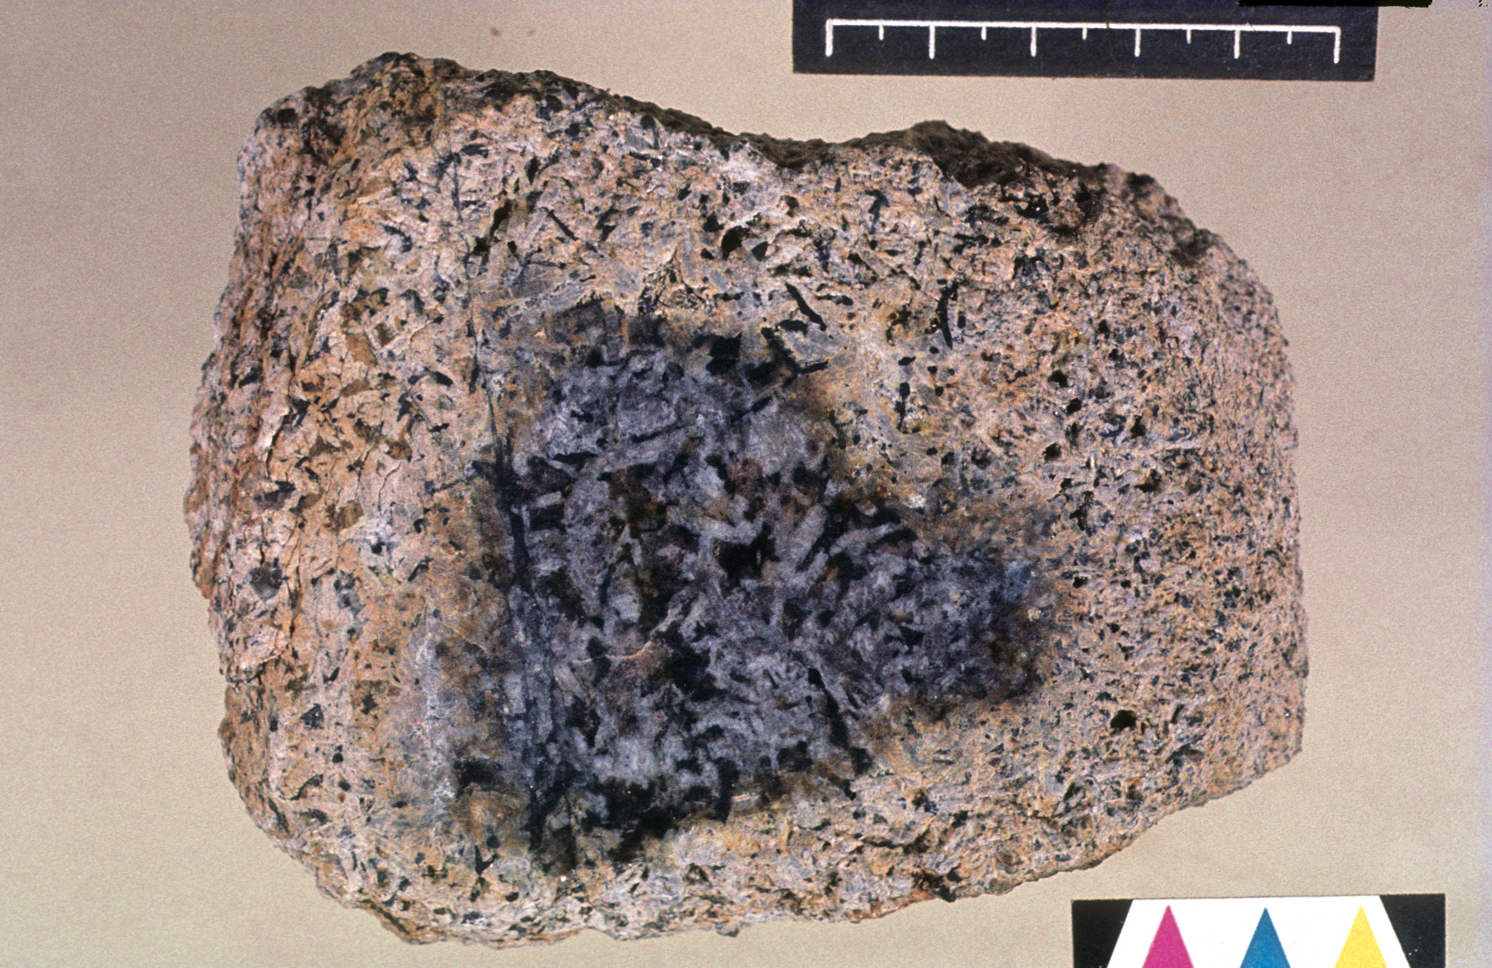
\includegraphics[width=\linewidth,height=4.6cm,keepaspectratio]{images/book1/bauxite.jpg}

{\small बॉक्साइट, ऐलुमिनियम का \omterm{def:g5:raw-materials-and-recycling:raw-material}{अयस्क}, अपक्षय से बची चट्टान के एक क्रोड के
चारों ओर। फ़ोटो: वेर्नर शेलमान, CC BY-SA 2.5।}
\end{minipage}\hfill
\begin{minipage}[b]{0.48\linewidth}\centering
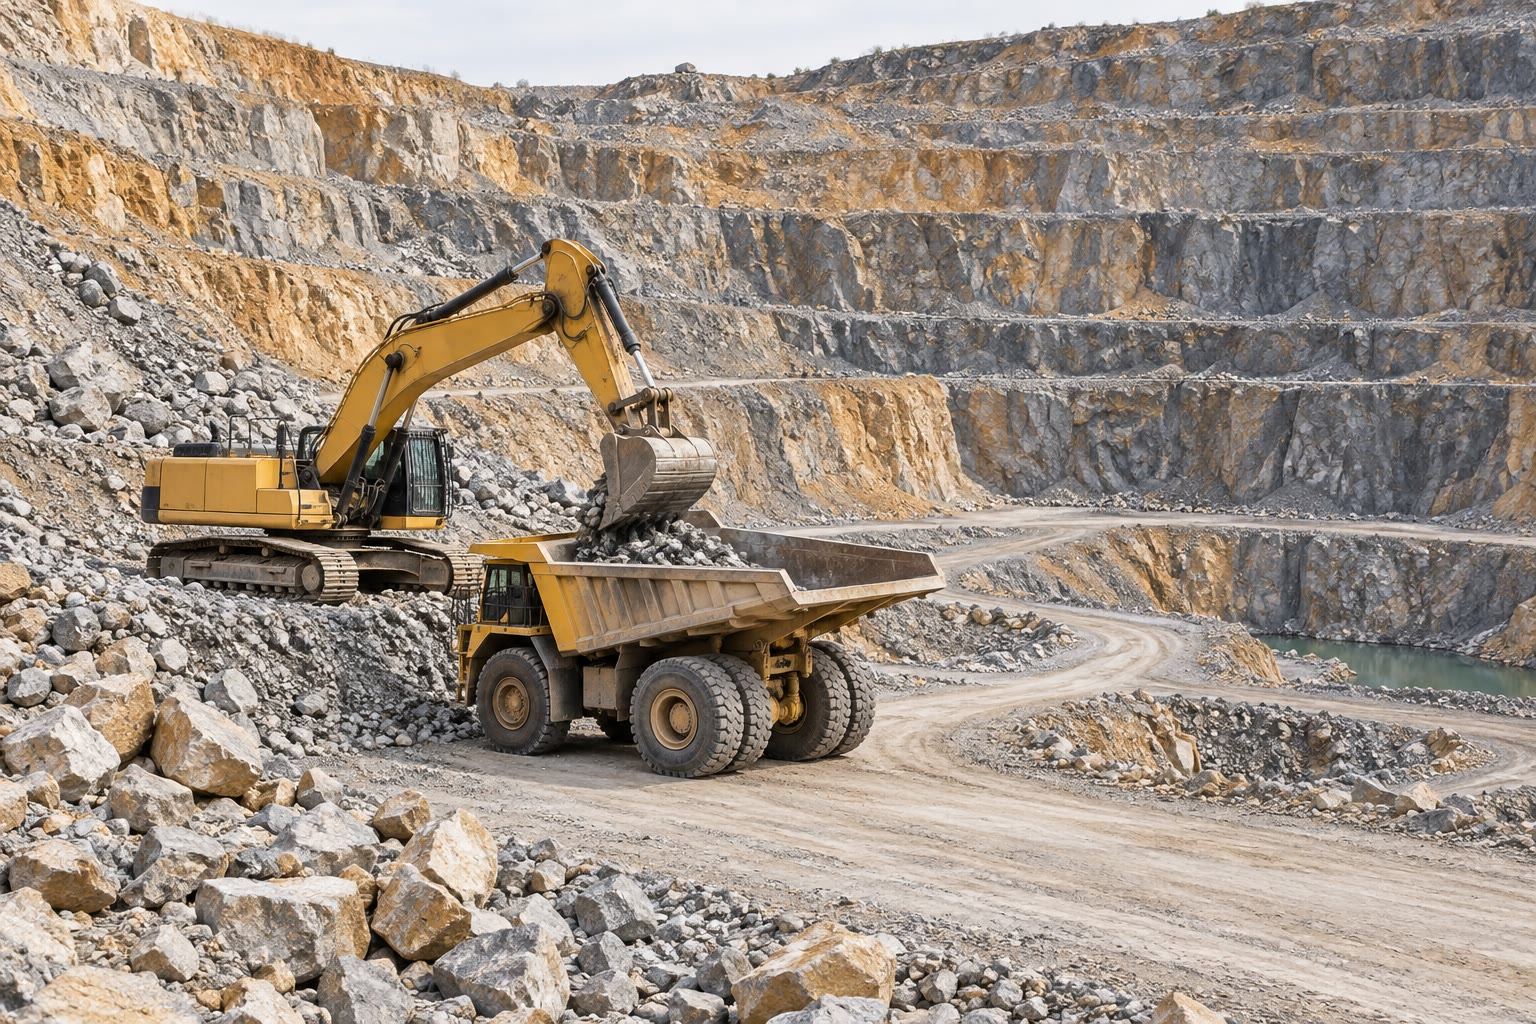
\includegraphics[width=\linewidth,height=4.6cm,keepaspectratio]{images/book1/ai/g5-quarry.jpg}

{\small खदान: चट्टान खोदकर निकाली जाती है ताकि कच्चे माल के रूप में काम आए।}
\end{minipage}
\end{omfigure}

\begin{omfigure}
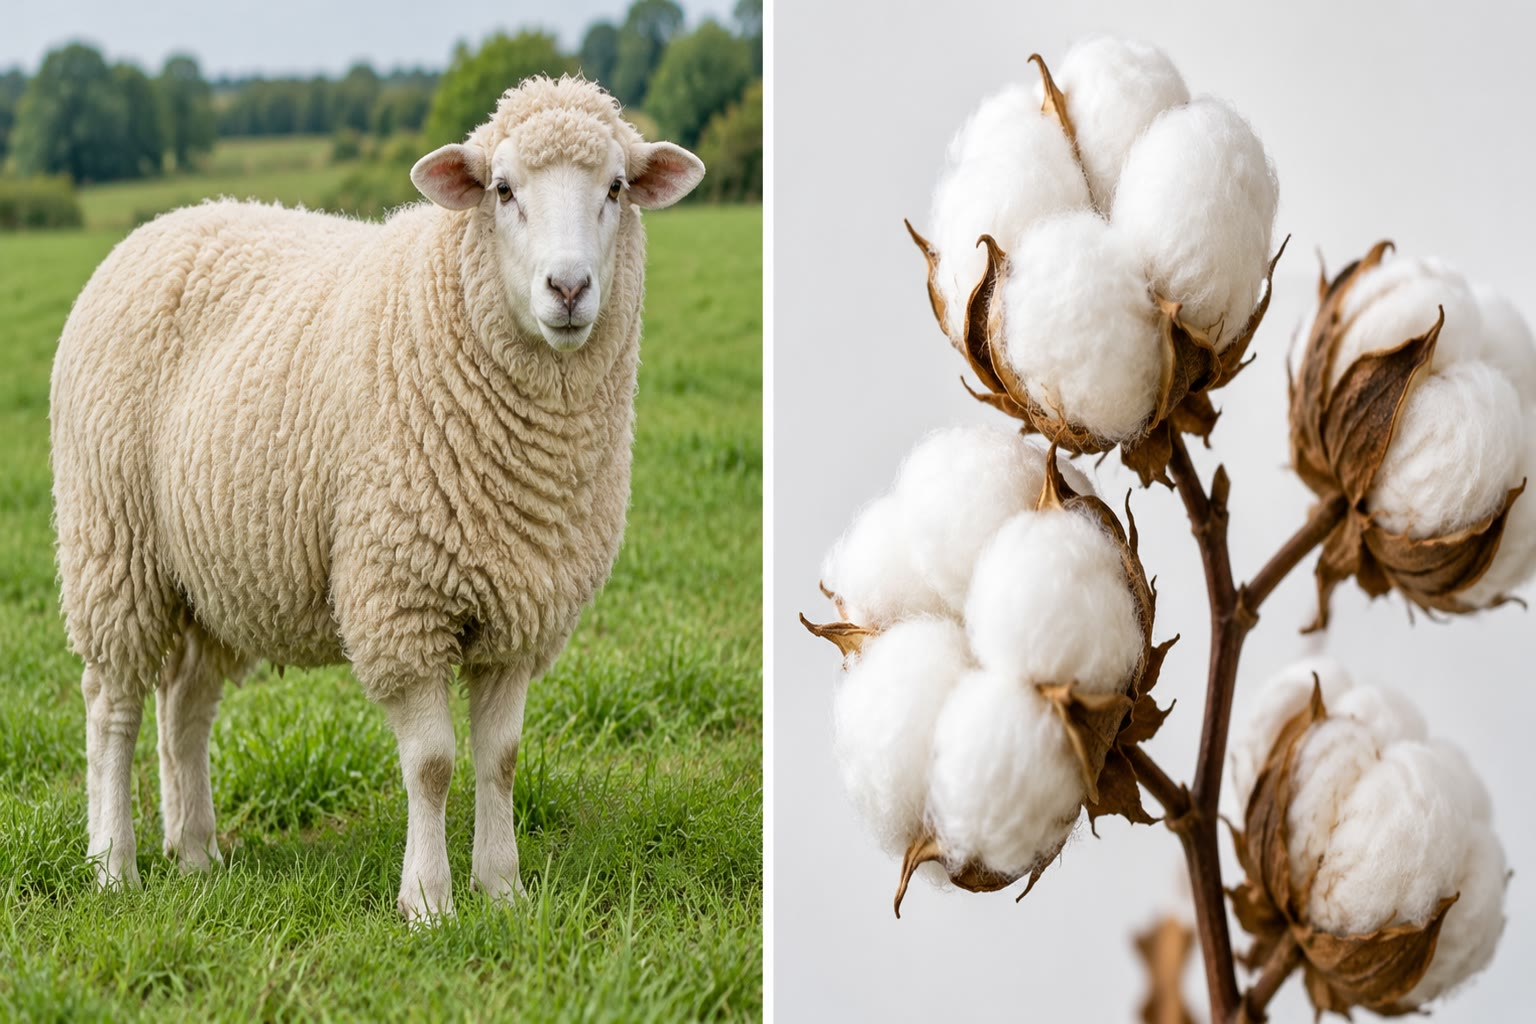
\includegraphics[width=0.6\linewidth]{images/book1/ai/g5-sheep-cotton.jpg}

{\small सजीवों से मिलने वाला प्राकृतिक \omterm{def:g5:raw-materials-and-recycling:raw-material}{कच्चा माल}: भेड़ों से ऊन,
कपास के पौधे से कपास।}
\end{omfigure}

\section{कच्चे माल से वस्तु तक}

\begin{proposition}[सामग्री बनाने से उसका कच्चा माल बदल जाता है]\label{prop:g5:raw-materials-and-recycling:change}
कच्चे माल को \omterm{def:g5:raw-materials-and-recycling:natural-material}{निर्मित सामग्री} में बदलने के लिए ऊर्जा चाहिए ---
ज़्यादातर भट्ठी की ऊष्मा --- और आम तौर पर \omterm{def:g5:irreversible-changes:chemical-change}{रासायनिक परिवर्तन} होते हैं: रेत
काँच बन जाती है, \omterm{def:g5:raw-materials-and-recycling:raw-material}{अयस्क} धातु, तेल प्लास्टिक। इन परिवर्तनों को सीधे-सीधे
उलटा नहीं किया जा सकता: काँच वापस रेत नहीं बनता।
\end{proposition}

\begin{example}[काँच की बोतल का जीवन]\label{ex:g5:raw-materials-and-recycling:bottle}
रेत, सोडा और पिसा हुआ चूना पत्थर एक भट्ठी में साथ-साथ तब तक गरम किए जाते
हैं जब तक वे पिघलकर काँच नहीं बन जाते। गरम काँच को फूँककर बोतल का आकार
दिया जाता है। बोतल भरी जाती है, बिकती है और ख़ाली होती है। काँच के
कूड़ेदान में डालने पर उसे तोड़कर छोटे टुकड़े किए जाते हैं, फिर से पिघलाया जाता
है और फूँककर नई बोतल बनाई जाती है: काँच बार-बार काम आता है।
\end{example}

\begin{omfigure}
\begin{tikzpicture}[font=\small,
    box/.style={draw=omDef, fill=omDef!6, rounded corners=2pt, align=center,
      minimum height=0.95cm, text width=2.4cm}]
  \node[box] (r) at (0,2.6) {कच्चा माल\\ (रेत, अयस्क, तेल)};
  \node[box] (m) at (4.0,2.6) {सामग्री\\ बनाना};
  \node[box] (o) at (8.0,2.6) {वस्तु,\\ उपयोग में};
  \node[box] (w) at (8.0,0) {कचरा};
  \node[box, draw=omProp, fill=omProp!8] (s) at (4.0,0) {छँटाई और\\ पुनर्चक्रण};
  \draw[->, thick, omDef] (r) -- (m);
  \draw[->, thick, omDef] (m) -- (o);
  \draw[->, thick, omDef] (o) -- (w);
  \draw[->, thick, omProp] (w) -- (s);
  \draw[->, thick, omProp] (s) -- (m) node[midway, left, align=right, text=black]
    {नए कच्चे माल\\ की जगह फिर\\ से उपयोग};
  \draw[->, thick, black!45, dashed] (w.east) -- ++(1.4,0) node[right, align=left,
    text=black] {फेंक दिया:\\ भराव-स्थल};
\end{tikzpicture}

{\small किसी सामग्री का जीवन। नारंगी चक्र \omterm{def:g5:raw-materials-and-recycling:recycling}{पुनर्चक्रण} है: पुरानी वस्तु की
सामग्री नए कच्चे माल की जगह लेती है।}
\end{omfigure}

\section{छँटाई और पुनर्चक्रण}

\begin{definition}[पुनर्चक्रण]\label{def:g5:raw-materials-and-recycling:recycling}
\emph{पुनर्चक्रण}\index{पुनर्चक्रण} यानी इस्तेमाल हो चुकी वस्तुओं को
इकट्ठा करना और उनकी सामग्री को इस तरह उपचारित करना कि उससे नई वस्तुएँ
बन सकें, बजाय उन्हें फेंक देने के।
\end{definition}

\begin{proposition}[पुनर्चक्रण क्यों]\label{prop:g5:raw-materials-and-recycling:why}
% ledger: al:energy-primary, al:energy-recycled (8.3 / 186 = about 1/22)
\omterm{def:g5:raw-materials-and-recycling:recycling}{पुनर्चक्रण} कच्चे माल को बचाता है, जिसे ज़मीन से खोदकर नहीं निकालना पड़ता,
और अक्सर ऊर्जा भी बचाता है। पुराने डिब्बों से ऐलुमिनियम बनाने में उस ऊर्जा
का केवल लगभग बीसवाँ भाग लगता है जो उसे बॉक्साइट से बनाने में लगती है।
इसका अर्थ यह भी है कि भराव-स्थलों में कम कचरा जाता है।
\end{proposition}

\begin{method}[पुनर्चक्रण के लिए कचरा छाँटना]\label{met:g5:raw-materials-and-recycling:sort}
\omterm{def:g5:raw-materials-and-recycling:recycling}{पुनर्चक्रण} छँटाई से शुरू होता है, जहाँ भी कचरा फेंका जाता है:
\begin{enumerate}
  \item काँच की बोतलें और मर्तबान एक कूड़ेदान में;
  \item धातु के डिब्बे, कागज़ और गत्ता, और प्लास्टिक की बोतलें उन कूड़ेदानों
        में जो नगर ने उनके लिए रखे हैं (कूड़ेदानों के रंग जगह-जगह
        अलग होते हैं);
  \item जो पुनर्चक्रित नहीं हो सकता, वह बाकी कचरे के साथ।
\end{enumerate}
हर सामग्री का \omterm{def:g5:raw-materials-and-recycling:recycling}{पुनर्चक्रण} अपने ढंग से होता है, इसलिए किसी कूड़ेदान में
केवल वही सामग्रियाँ होनी चाहिए जिनके लिए वह बना है।
\end{method}

\begin{omfigure}
\begin{tikzpicture}[font=\small]
  \foreach \k/\t/\bc in {0/काँच/green!50!black, 1/{धातु के डिब्बे}/gray,
                        2/{कागज़ और गत्ता}/omDef, 3/{प्लास्टिक की बोतलें}/orange!80!black} {
    \begin{scope}[xshift=\k*3.4cm]
      \fill[\bc!18, draw=\bc, line width=0.8pt] (-1,0) -- (1,0) -- (1.15,2.0)
        -- (-1.15,2.0) -- cycle;
      \fill[\bc!45, draw=\bc] (-1.25,2.0) rectangle (1.25,2.3);
      \node[anchor=north, align=center] at (0,-0.15) {\t};
    \end{scope}
  }
  % glass: a bottle
  \fill[green!40!black!60] (-0.2,0.3) rectangle (0.2,1.2);
  \fill[green!40!black!60] (-0.07,1.2) rectangle (0.07,1.6);
  % metal: a can
  \begin{scope}[xshift=3.4cm]
    \fill[black!25, draw=black!55] (-0.3,0.3) rectangle (0.3,1.3);
  \end{scope}
  % paper: a box and a sheet
  \begin{scope}[xshift=6.8cm]
    \fill[brown!25, draw=brown!60] (-0.6,0.3) rectangle (0.1,1.0);
    \fill[white, draw=black!40] (0.2,0.3) rectangle (0.65,1.3);
  \end{scope}
  % plastic: a bottle
  \begin{scope}[xshift=10.2cm]
    \fill[cyan!20, draw=cyan!50!black] (-0.25,0.3) rectangle (0.25,1.3);
    \fill[cyan!20, draw=cyan!50!black] (-0.1,1.3) rectangle (0.1,1.6);
  \end{scope}
\end{tikzpicture}

{\small चार छँटाई कूड़ेदान, हर सामग्री के लिए एक। (असली कूड़ेदानों के रंग
एक नगर से दूसरे नगर में अलग होते हैं।)}
\end{omfigure}

\begin{omfigure}
\begin{minipage}[t]{0.48\linewidth}\centering
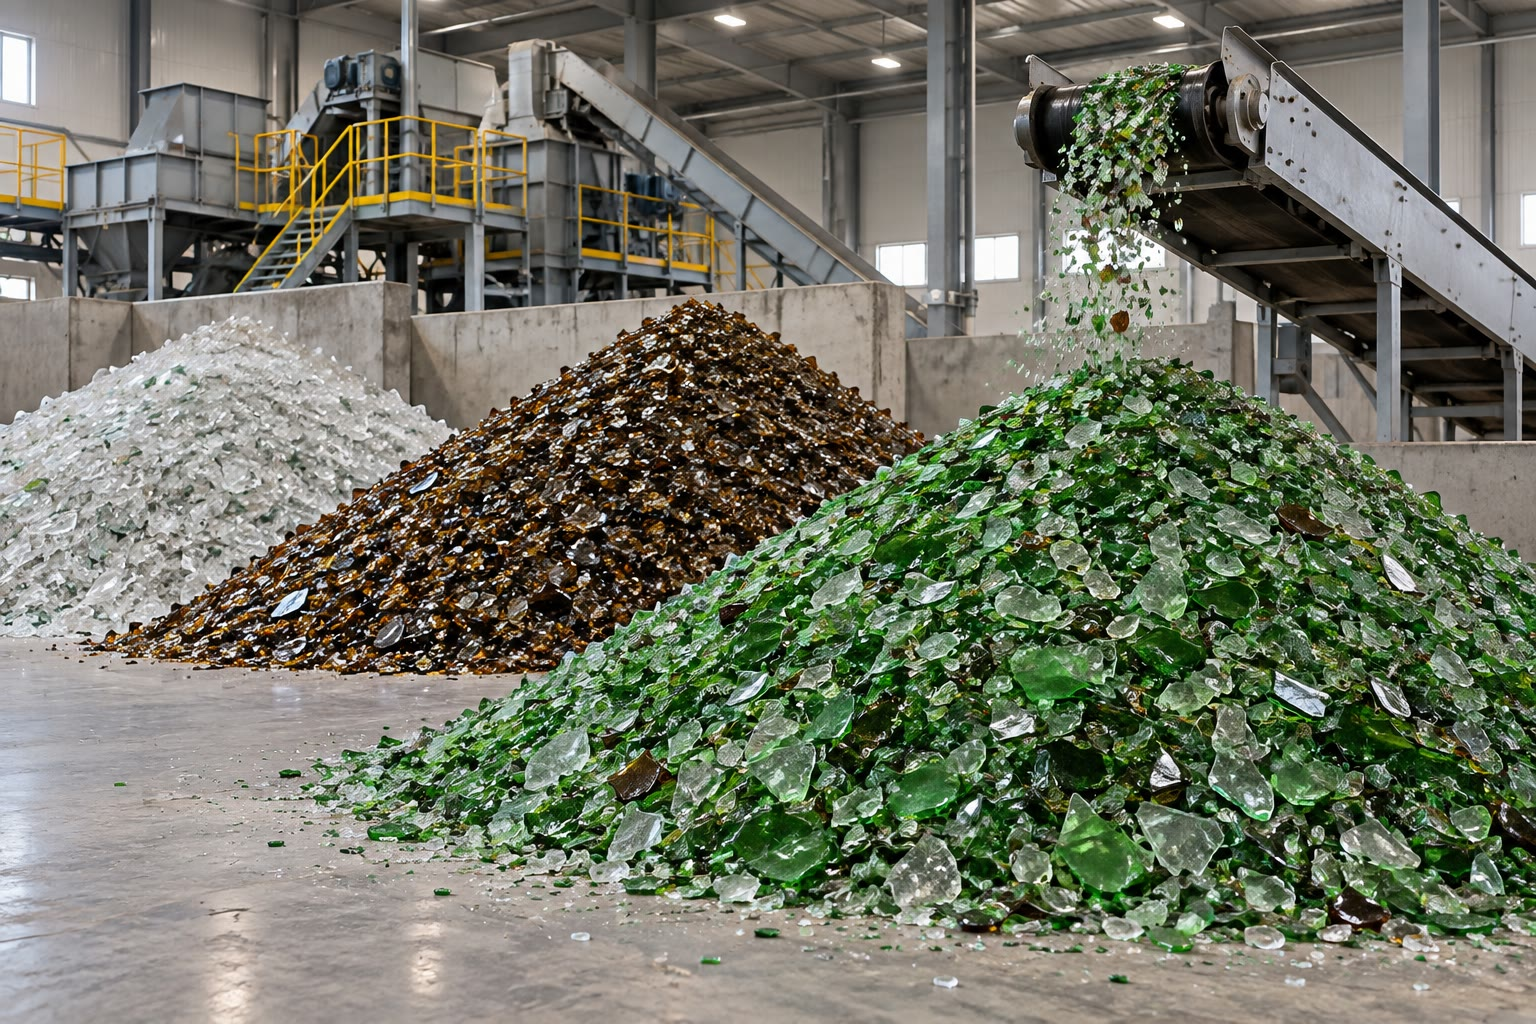
\includegraphics[width=\linewidth,height=4.6cm,keepaspectratio]{images/book1/ai/g5-glass-cullet.jpg}

{\small \omterm{def:g5:raw-materials-and-recycling:recycling}{पुनर्चक्रण} संयंत्र में तोड़ा हुआ काँच, पिघलाए जाने को तैयार।}
\end{minipage}\hfill
\begin{minipage}[t]{0.48\linewidth}\centering
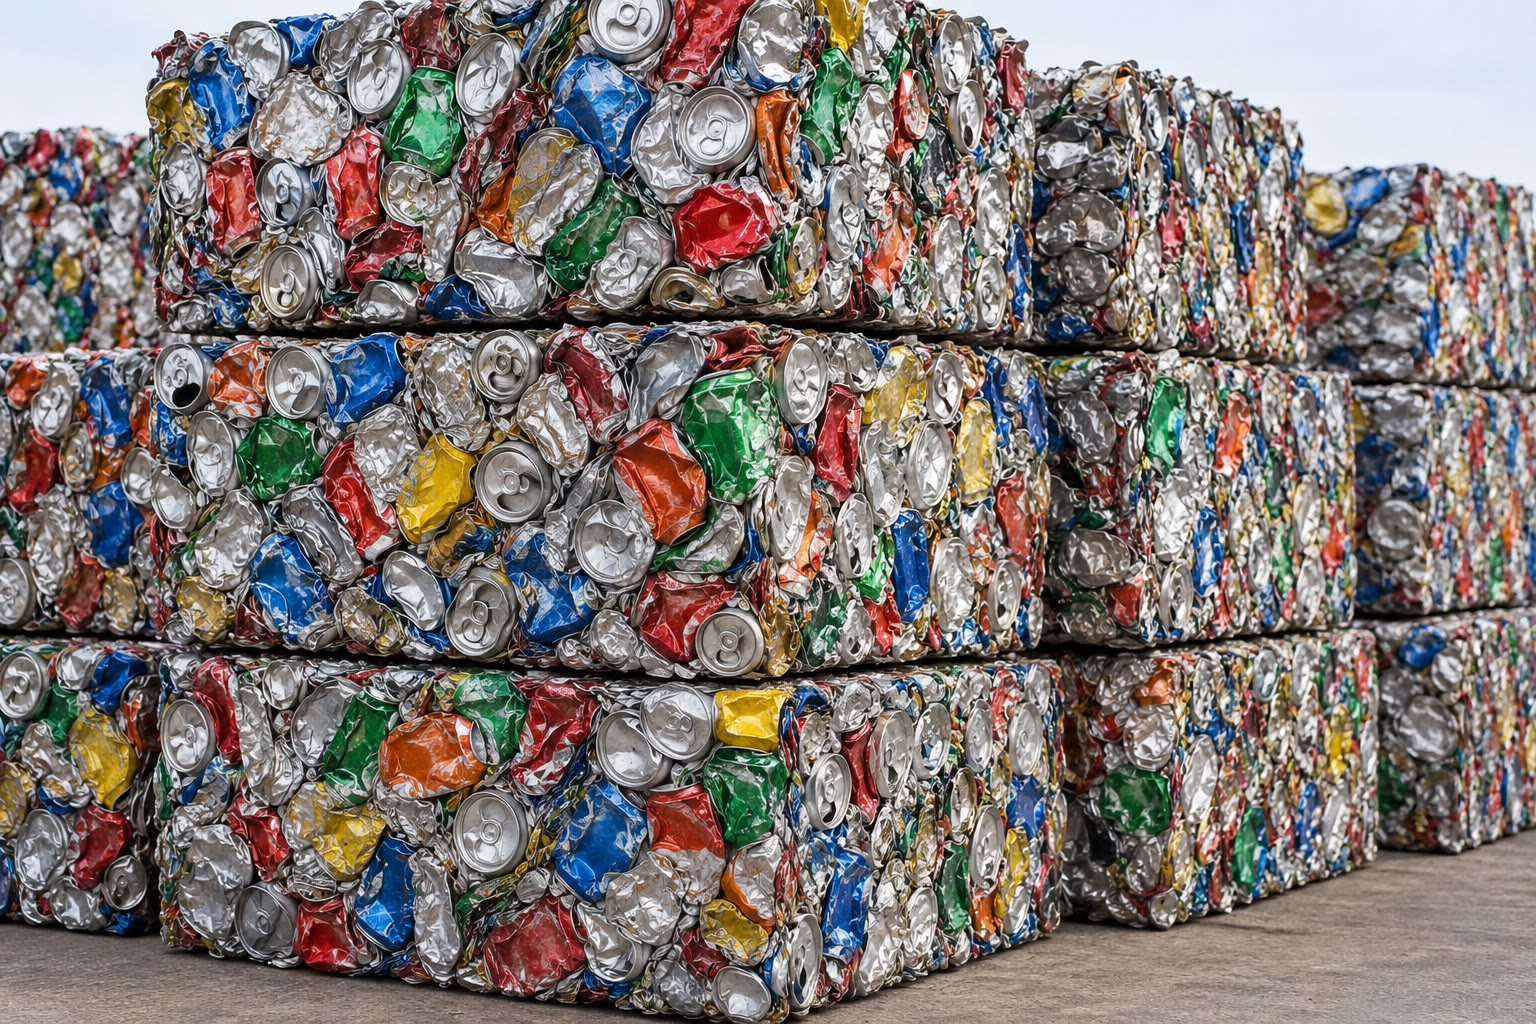
\includegraphics[width=\linewidth,height=4.6cm,keepaspectratio]{images/book1/ai/g5-can-bales.jpg}

{\small ऐलुमिनियम के दबाए हुए डिब्बों के गट्ठर।}
\end{minipage}
\end{omfigure}

\section{कचरा और संसाधन}

\begin{definition}[संसाधन]\label{def:g5:raw-materials-and-recycling:resource}
\emph{संसाधन}\index{संसाधन} प्रकृति से ली गई कोई भी चीज़ है जिसका
मनुष्य उपयोग करते हैं: पानी, लकड़ी, \omterm{def:g5:raw-materials-and-recycling:raw-material}{अयस्क}, तेल, रेत। \emph{नवीकरणीय
संसाधन}\index{नवीकरणीय संसाधन} मनुष्य के जीवनकाल के भीतर अपने आप फिर से
उग आता या लौट आता है, जैसे फिर से पेड़ लगाए गए जंगल की लकड़ी या भेड़ों
की ऊन। \omterm{def:g5:raw-materials-and-recycling:raw-material}{अयस्क} और कच्चा तेल नवीकरणीय नहीं हैं: एक बार खोदकर निकाल लिए
और इस्तेमाल हो गए, तो वे ख़त्म हो जाते हैं।
\end{definition}

\begin{proposition}[कम करो, फिर से उपयोग करो, पुनर्चक्रण करो]\label{prop:g5:raw-materials-and-recycling:three}
\omterm{def:g5:raw-materials-and-recycling:resource}{संसाधनों} को लंबे समय तक चलाने के लिए लोग, इसी क्रम में, यह कर सकते हैं:
\begin{enumerate}
  \item \textbf{कम करना}: कम वस्तुएँ इस्तेमाल करना, जैसे कम
        पैकिंग;
  \item \textbf{फिर से उपयोग करना}: उसी वस्तु को दोबारा काम में लेना, जैसे
        फिर से भरा गया काँच का मर्तबान या दुकान पर वापस ले जाया गया थैला;
  \item \textbf{\omterm{def:g5:raw-materials-and-recycling:recycling}{पुनर्चक्रण} करना}: सामग्री से एक नई वस्तु बनाना।
\end{enumerate}
\omterm{def:g5:raw-materials-and-recycling:recycling}{पुनर्चक्रण} सबसे आख़िर में आता है, क्योंकि उसमें भी ऊर्जा और मशीनें लगती
हैं; सबसे अच्छा कचरा वह है जो कभी बने ही नहीं।
\end{proposition}

\section{अभ्यास}

\begin{exercise}[$\star$]\label{exo:g5:raw-materials-and-recycling:1}
प्राकृतिक या निर्मित? लकड़ी, काँच, ऊन, स्टील, प्लास्टिक, पत्थर।
\end{exercise}

\begin{exercise}[$\star$]\label{exo:g5:raw-materials-and-recycling:2}
इनका \omterm{def:g5:raw-materials-and-recycling:raw-material}{कच्चा माल} बताओ: कागज़ का पन्ना, काँच का मर्तबान, सूती
टी-शर्ट, प्लास्टिक की बोतल।
\end{exercise}

\begin{exercise}[$\star$]\label{exo:g5:raw-materials-and-recycling:3}
\omterm{def:g5:raw-materials-and-recycling:raw-material}{अयस्क} क्या है? ऐलुमिनियम के \omterm{def:g5:raw-materials-and-recycling:raw-material}{अयस्क} का नाम बताओ।
\end{exercise}

\begin{exercise}[$\star$]\label{exo:g5:raw-materials-and-recycling:4}
तुम इन्हें किस कूड़ेदान में डालोगे: जैम का ख़ाली मर्तबान, अख़बार, पेय का डिब्बा,
पानी की प्लास्टिक बोतल?
\end{exercise}

\begin{exercise}[$\star$]\label{exo:g5:raw-materials-and-recycling:5}
किसी सामग्री के जीवन वाला चित्र देखो। नारंगी चक्र किसकी जगह
लेता है?
\end{exercise}

\begin{exercise}[$\star$]\label{exo:g5:raw-materials-and-recycling:6}
नवीकरणीय है या नहीं: लकड़ी, कच्चा तेल, ऊन, लौह \omterm{def:g5:raw-materials-and-recycling:raw-material}{अयस्क}, कपास?
\end{exercise}

\begin{exercise}[$\star$]\label{exo:g5:raw-materials-and-recycling:7}
काँच को ठंडा करके वापस रेत क्यों नहीं बनाया जा सकता?
\end{exercise}

\begin{exercise}[$\star$]\label{exo:g5:raw-materials-and-recycling:8}
कम करने का एक तरीका, फिर से उपयोग करने का एक तरीका और \omterm{def:g5:raw-materials-and-recycling:recycling}{पुनर्चक्रण} का एक तरीका बताओ।
\end{exercise}

\begin{exercise}[$\star$]\label{exo:g5:raw-materials-and-recycling:9}
काँच के कूड़ेदान में केवल काँच ही क्यों होना चाहिए?
\end{exercise}

\begin{exercise}[$\star\star$]\label{exo:g5:raw-materials-and-recycling:10}
पुराने डिब्बों से ऐलुमिनियम बनाने में उस ऊर्जा का लगभग बीसवाँ भाग लगता है
जो उसे बॉक्साइट से बनाने में लगती है। एक कारख़ाना बॉक्साइट से ऐलुमिनियम का
एक खेप बनाने में ऊर्जा की 20 इकाइयाँ खर्च करता है। वही खेप पुराने डिब्बों से
बनाने में लगभग कितनी इकाइयाँ लगेंगी?
\end{exercise}

\begin{exercise}[$\star\star$]\label{exo:g5:raw-materials-and-recycling:11}
``कम करना'' को ``\omterm{def:g5:raw-materials-and-recycling:recycling}{पुनर्चक्रण}'' से पहले क्यों रखा गया है?
\end{exercise}
